\externaldocument{../3/chapter_modeling}
\externaldocument{../5/chapter_implementation}
\externaldocument{../appendix/chapter_app}
\startchapter{Communication Identification Algorithms}
\label{chapter:alo}
The goal of this work is to identify the communications from the dual\_trace. A dual\_trace is a pair of assembly level execution traces of two interacting programs. In this chapter, I discuss the characteristics of the execution trace and give the abstract definition of the execution trace. Based on the communication model in Chapter\ref{chapter:Mod}, I developed the algorithms for communication identification from dual\_trace. Traces captured by different tracers can be analyzed with these developed algorithms, as long as the traces comply the abstract trace definition.

\section{Dual\_Trace}
A dual\_trace consists of two assembly level execution traces of two interacting programs. There is no timing information of these two traces which means we don't know the timing relationship of the events of one trace with respect to the other. However the captured instructions in the trace are ordered in execution sequence. An execution trace consist of a sequence of executed instruction lines. Each instruction line contains the executed instruction, the changed memories, the changed registers, execution information. The execution info indicate the execution type which can be: Instruction, System call entry, System call exit, etc. For the execution type of system call entry and system call exit, system call Id is given in this information. With the system call id and the provided .dll files, the called system function name can be obtained. 

Based on the characteristics of the execution trace, a dual\_trace is defined as :

$dual\_trace = \lbrace trace_0, trace_1\rbrace$

where $trace_0$ and $trace_1$ are two assembly execution traces of two interacting programs.

A trace is a sequence of executed instruction line. Hence, we can define a trace $trace$ as a sequence of $n$ instruction lines:

$ trace = (l_1, l_2, ..., l_n)$ 

Each instruction line, $l$ is a tuple:

$l = <ins, mch, rch, exetype, syscallInfo>$

where $ins$ is the instruction, $mch$ is the memory changes, $rch$ is the register changes, $exetype$ is the execution type which can be instruction, system call entry, system call exit, and other types which are not concerned, $syscallInfo = <exeName, offset>$ only appear when $exetype$ is system call entry or system call exit. $exeName$ is the executable file(e.g .dll and .exe) name, while $offset$ is the offset of the system function in this executable file.

Figure\ref{trace} is an example of a piece of execution trace comply to this definition. Some executed instructions are hidden to highlight the characteristic of the trace. 

\begin{figure}[H]
\centerline{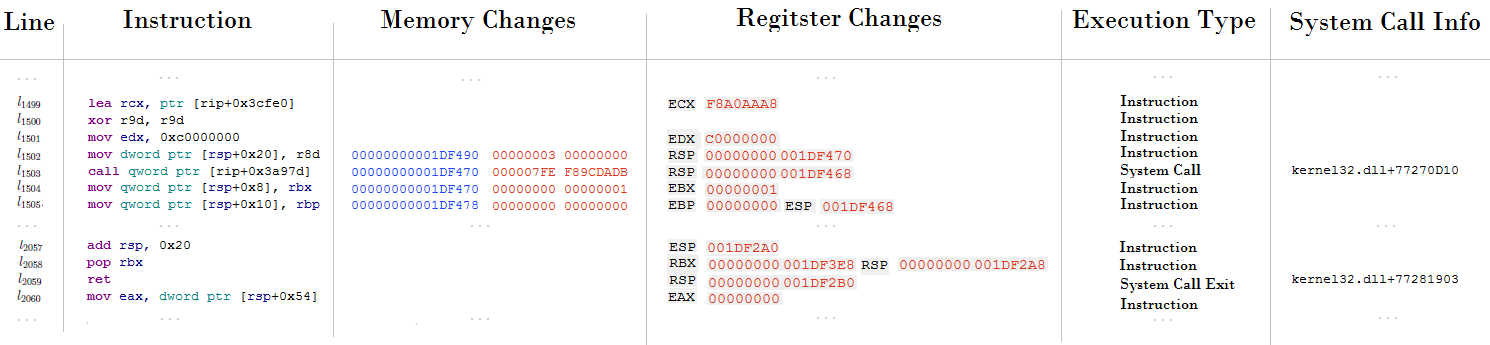
\includegraphics[scale=0.5]{Figures/trace}}
\caption{An example trace }
\label{trace}
\end{figure}

Figure\ref{executable} is an example of the information decoded from a executable file kernal32.dll, from which the function name can be obtained by the offset.

\begin{figure}[H]
\centerline{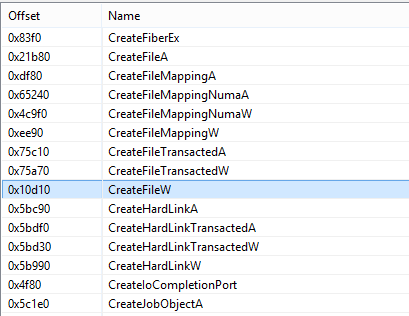
\includegraphics{Figures/executable}}
\caption{Information of kernal32.dll}
\label{executable}
\end{figure}

\section{Function Event Reconstruction Algorithm}
In last section, I define the assembly execution trace. As to this definition, it is possible to recognize the function call and function call return from the trace.  In this section, I define the function event and discuss the algorithm to reconstruct the function events from the assembly execution trace. 


There would be lots of function calls in an execution trace while most of them are not of interest. This algorithm will only reconstruct those function calls of interest. To be able to identify the functions of interest, function descriptions is required. The function descriptions $fdes$ are:

A list of function descriptions of a communication method, each description includes a function name, a function type indicator and a function description. The function type indicator is marked as one of the four types: open, close, send and receive events. This indicator is not needed in this algorithm but will be used in the stream extraction algorithm. The function description illustrate how the current registers and memory contents map to a given function call and the list of its parameter of interest(you might not care for all parameters). 

Table\ref{functionexample} is an example of an element in the function descriptions. In this example, the function name is ReadFile, it is a function for data receiving. The description includes the concerned parameters, which are File Handle, Send Buffer and Message Length. The File Handle is a input parameter which is a value stored in the register RCX. The Send Buffer is an address for the input message stored in the register RAX. The Message Length is a output value stored in register R9. The value of the input parameters can be retrieved from the memory reconstruction on the function call instruction line while the value of the output parameters can be retrieved from the memory reconstruction on the function return instruction line. If a parameter is a address instead of value, the address should be retrieved first, then the retrieved address should be used to find the buffer content in the memory reconstruction result as well.  The function description requires the understanding of the calling convention of the operating system. More example will be given in Chapter\ref{chapter:newsol}.

\begin{table}[H]
        \centering
        \caption{An example of a function description}
        \label{functionexample}
        \begin{tabular}{|l|l|l|l|l|l|}
            \hline
             \multirow{2}{*}{{\textbf{Name}}} & \multirow{2}{*}{{\textbf{Type}}} & \multicolumn{4}{c|}{\textbf{Description}}  \\
              \cline{3-6} 
             & & \textbf{Parameter}& \textbf{Register/Stack Position}& \textbf{In or Out} &  \textbf{Buffer Or Value}  \\
             \hline
             \multirow{3}{*}{ReadFile}
             &\multirow{3}{*}{data receive} &  Handle & RCX & In & Value\\
              \cline{3-6} 
             & & SendBuffer & RDX & In & Address\\
              \cline{3-6} 
             & & MessageLength & R9 & Out & Value\\
            \hline            
        \end{tabular}
    \end{table}

With the function descriptions and the execution trace as input, the function event reconstruction algorithm outputs all the function call events from the execution trace. A function call event is defined as a tuple:

$ev = <funN, paras, type>$

where $funN$ is the function name, $paras$ includes all the input/output parameters and the return value, and $type$ is the event type which can be one of the four types: open, send, receive and close.

Note: if the parameter is an address, the value is the string from the buffer pointed by this address instead of the address value.

The output of the function event reconstruction algorithm $etr$ is a size $m$ sequence of function call events which can be defined as:

$etr = (ev_1, ev_2, ..., ev_m)$

An example of a sequence of function call events as the output of this algorithm is shown in Listing\ref{eventsexample}.

\begin{lstlisting}[caption= Example of  $etr$, label=eventsexample]
{funN:CreateNamedPipe, paras:{Handler:18, FileName:mypipe}, type:open},
{funN:CreateNamedPipe,  paras:{Handler:27,  FileName:Apipe}, type:open},
{funN:WriteFile, paras:{Handler:27, RecvBuffer:Message1, MessageLength:9}, type:send},
{funN:WriteFile, paras:{Handler:27, RecvBuffer:Message2, MessageLength:9}, type:send},
{funN:ReadFile, paras:{Handler:27, SendBuffer:Message3, MessageLength:9}, type:receive},
{funN:CloseHandle, paras:{Handler:27}, type:close},
{funN:CloseHandle, paras:{Handler:18}, type:close}
\end{lstlisting}

The function event reconstruction algorithm is listed in Algorithm\ref{eventAlg}. This algorithm is designed for reconstruct the function call events of a communication method. If multiple communication methods are under investigated, this algorithm can be run multiple times to achieve the goal. Since the function descriptions usually contain a  small number of concerned functions compared to the instruction line number in the execution trace, the time complexity of this algorithm is O(N) , N is the instruction line number of the trace.

\begin{algorithm}[H]
\DontPrintSemicolon
\caption{{\bf Function Event Reconstruction Algorithm} \label{eventAlg}}
\KwIn{ $trace, fdes$}
\KwOut{$etr$}
$etr \leftarrow \emptyset$\; 
Emulate the Execute of each instruction line of the trace;\;
\If{The instruction is a call to a function in the $fdes$}{
   Create an new function call event $ev$;\;
   $ev.funN  \leftarrow$ Function Name from the $fdes$;\;
   $ev.type  \leftarrow$ Function Type from the $fdes$;\;
   Append all the input parameters of interest to $ev.paras$;\;
   Continue the emulation until the function call return line;\;
   Append all the output parameters of interest to $ev.paras$;\;
   Append $ev$ to $etr$;\;
}
\KwRet $etr$;\;
\end{algorithm} 


\section{Stream Extraction}
The function call events in the $etr$ may belong to different streams. A stream is a size $k$ sequence of function call events correspond to the same endpoint of a communication which can be defined as:

$s = (ev_1, ev_2, ..., ev_k)$

Note: the definition of $ev$ in $s$ is identical to the that in $etr$. However, the event numbering of $s$ is different from $etr$. For example, $ev_1$ in $s$ and $ev_1$ in $etr$ might be different events.

The stream extraction algorithm is designed to extract the streams from the sequence of function call events. In this algorithm, the stream is need to be identify by the channel open function calls first. Then all other events related to this stream will be added to the stream.

\subsection{Channel Open Mechanisms}
The channel open mechanism affect the stream identification strategy. The channel open mechanism of named pipe and message queue is relatively simple. In windows implementation, only one function call is related to the handle identification of the stream. However, for TCP and UDP the mechanism is slightly complicated.

\subsubsection{Named Pipe Channel Open Mechanisms} 
A named pipe server is responsible for the creation of the pipe, while clients can connect to the pipe after it was created. The creation and connection of a named pipe returns the Filehandle of that pipe. So the identification of the stream only need to identify the pipe creation function call on the server side and the pipe connection function call on the client side. The Filehandle returned by these function calls will be used later when data is being sent or received to a specified pipe. Figure\ref{namedpipeopen} exemplify the channel set up process for a Named Pipe communication in Windows. 

\begin{figure}[H]
\centerline{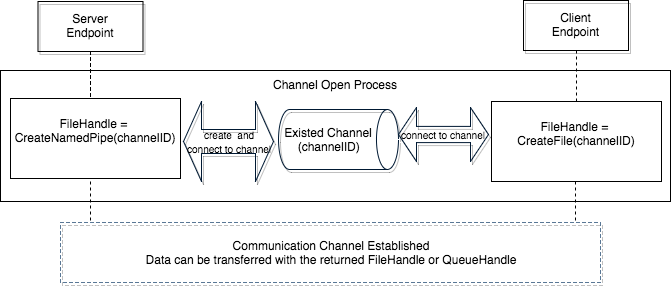
\includegraphics[scale=0.55]{Figures/namepipechannelopen}}
 \caption{Channel Open Process for a Named Pipe in Windows}
\label{namedpipeopen}
\end{figure}
    
\subsubsection{Message Queue Channel Open Mechanisms} 
For the Message Queue communication method, the endpoints of the communication can create the queue or use the existing one. However, both of them have to open the queue before they access it. The QueueHandle returned by the open queue function will be used later on when messages are being sent or received to identify the queue. Figure\ref{msmqopen} exemplify the channel set up process for a Message Queue communication in Windows.
\begin{figure}[H]
\centerline{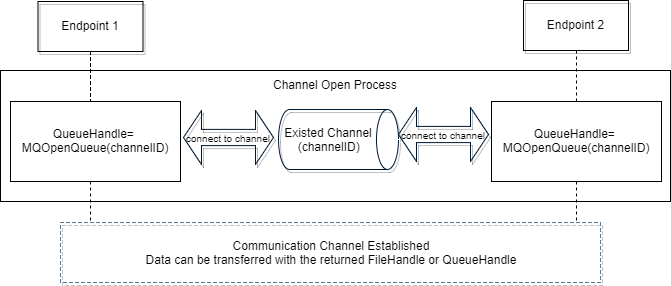
\includegraphics[scale=0.55]{Figures/msmqchannelopen}}
 \caption{Channel Open Process for a Message Queue in Windows}
\label{msmqopen}
\end{figure}

\subsubsection{UDP and TCP Channel Open Mechanisms} 
The communication channel is set up by both of the endpoints for UDP and TCP channels. The function \textit{socket} should be called to create their own socket on both endpoints. After the socket handle are created, the server endpoint binds the socket to its service address and port by calling the function \textit{bind}. Then the server endpoint calls the function  \textit{accept} to accept the client connection. The client will call the function \textit{connect} to connect to the server. When the function \textit{accept} return successfully, a new socket handle will be generated and returned for further data transfer between the server endpoint and  the connected client endpoint. After all these operations are performed successfully, the channel is established and the data transfer can start. During the channel open stage, server endpoint has two socket handles, the first one is used to listen to the connection from the client, while the second one is created for real data transfer. Figure\ref{channelopen2} exemplify the channel open process for TCP and UDP  in Windows.
    
\begin{figure}[H]
\centerline{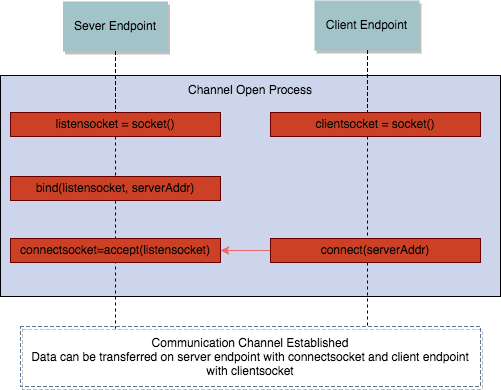
\includegraphics[scale=0.55]{Figures/tcpudpchannelopen}}
 \caption{Channel Open Model for TCP and UDP in Windows}
\label{channelopen2}    
\end{figure}

\subsection{Algorithm}
The input of this algorithm the $etr$ from the ``Function Event Reconstruction Algorithm" in Algorithm\ref{eventAlg}. Since the events in $etr$ are reconstructed in sequence of the instructions which are order by the time of occurrence, the events are implicitly sorted by time of occurrence. According to the relative time attribute in the communication model in Chapter\ref{chapter:Mod}, the open events should always happen before other events. So the stream can be identified by its channel open function call event. 

The output of this algorithm is a set of $s$ of size $l$, which can be defined as:
$str = (s_1, s_2, ..., s_l)$

As to the channel open mechanisms, two different algorithms are designed, one is for Name pipe and Message Queue, while the other is for TCP and UDP. For these communication, the handles which can be File Handle, Queue Handle and Socket Handle are represented as handle.

\subsubsection{Stream Extraction Algorithm for Named Pipe and Message Queue}
This algorithm is designed for extraction of the streams for Named Pipe and Message Queue. Since for each endpoint of the communication, only one channel open function call exist, it is simple to identify the stream starts once a channel open function call event is found. However, the handle of this stream reuse would not happen before this stream was closed by the channel close function call event. This algorithm handle this by having the $tempstream$ set to keep track of the streams that are still open. Once the stream was closed, the handle can be used by another stream.
\begin{algorithm}[H]
\DontPrintSemicolon
\caption{{\bf Stream Exatraction Algorithm for Named Pipe and Message Queue} \label{endpointIdentAlg}}
\KwIn{$etr$}
\KwOut{$str$} 
$str \leftarrow \emptyset$\; 
$tempstreams \leftarrow \emptyset$\; \tcp*[f]{store the temperate detected streams before their extraction complete}\;  
\For{$ev \in etr$}{
   $h \leftarrow$the handle identifier from $ev.paras$;\;
   \If{$ev.type = open$}{
      \If{$tempstreams[h]$ not exist}{\tcp*[f]{A handle would not be reused until the stream closed}\;  
         $tempstreams[h] \leftarrow$ a new $s$;\;
         $tempstreams[h].append(ev)$;\;
      }
      
   }
   \If{$ev.type = send$ Or $ev.type = receive$}{      
      \If{$tempstreams[h]$ exist}{
         $tempstreams[h].append(ev)$;\;
      }
   }
   \If{$ev.type = close$}{
      \If{$tempstreams[h]$ exist}{
         $tempstreams[h].append(ev)$;\;
         $str.append(tempstreams[h])$;\;        
         remove $tempstreams[h]$ from $tempstreams$;\;\tcp*[f]{A handle can be reused after the stream closed}\;
      }
   }         
}
\KwRet $str$;\;
\end{algorithm} 

\subsubsection{Stream Extraction Algorithm for TCP and UDP}
This algorithm is designed for extraction of the streams for Named Pipe and Message Queue. mechanism of TCP and UDP is a bit complex. A socket handle created by function call of $socket$ for listening on the server is not the one that created by the function call of $accept$ for the data transmission. In the server side, the socket handle for listening can be treated the one of a parent stream, while the socket handle for data transmission can be treated as the child stream. The parent stream can generate multiple children sockets. The algorithm will only extract the children stream, but store the parent stream in $tempstreas$ for temperate usage. However the events in the parents stream contain the information needed for stream matching algorithm later, so the children stream will inherit all the events from their parent. In the client side, the parent socket and the child socket are the same one. All the socket handle can not be reused before the stream is closed.
\begin{algorithm}[H]
\DontPrintSemicolon
\caption{{\bf Stream Exatraction Algorithm for Named Pipe and Message Queue} \label{endpointIdentAlg}}
\KwIn{$etr$}
\KwOut{$str$} 
$str \leftarrow \emptyset$\; 
$tempstreams \leftarrow \emptyset$\; \tcp*[f]{store the temperate detected streams before their extraction complete}\;  
\For{$ev \in etr$}{
   \If{$ev$ is a function call to $socket$}{
      $h \leftarrow$ the handle identifier from $ev.paras$;\;
      \If{$tempstreams[h]$ not exist}{\tcp*[f]{A handle would not be reused until the stream closed}\;  
         $tempstreams[h] \leftarrow$ a new $s$;\;
         $tempstreams[h].append(ev)$;\;
      }     
   }
   
   \If{$ev$ is a function call to $bind$ or $connect$}{
      $h \leftarrow$ the handle identifier from $ev.paras$;\;
      \If{$tempstreams[h]$ exist}{
         $tempstreams[h].append(ev)$;\;
      }     
   }
   
   \If{$ev$ is a function call to $accept$}{
      $h \leftarrow$ the listen socket handle identifier from $ev.paras$;\;
      $hc \leftarrow$ the connect socket handle identifier from $ev.paras$;\;
      \If{$tempstreams[h]$ exist And $tempstreams[hc]$ not exist}{
         \tcp*[f]{create a new stream for the child stream}\;  
         $tempstreams[hc] \leftarrow$ a new $s$;\;
         \tcp*[f]{append all the events in the parent stream to the child stream}\;  
         $tempstreams[hc].append(tempstreams[h])$;\;
         \tcp*[f]{append the current event to the child stream}\;  
         $tempstreams[hc].append(ev)$;\;
      }     
   }
   
   
   \If{$ev.type = send$ Or $ev.type = receive$}{      
      \If{$tempstreams[h]$ exist}{
         $tempstreams[h].append(ev)$;\;
      }
   }
   \If{$ev.type = close$}{
      \If{$tempstreams[h]$ exist}{
         $tempstreams[h].append(ev)$;\;
         $str.append(tempstreams[h])$;\;        
         remove $tempstreams[h]$ from $tempstreams$;\;\tcp*[f]{A handle can be reused after the stream closed}\;
      }
   }         
}
\KwRet $str$;\;
\end{algorithm} 

\section{Stream Matching Algorithm}\label{streammatch}
The communication identification algorithm aims at identifying all the communication of a concerned communication method from the dual-trace. The input of this algorithm is the two $str$ from the dual-trace. The output of this algorithm is the communication list. Each communication recognized from the dual\_trace contains two streams. The channel of a communication defined in Section\ref{definition} is not explicitly represented in the output but it was implicitly used in this algorithm. 

In the communication identification algorithm, it first try to match two streams to a channel only by their identifiers. In this level, the matching depends on channel open mechanisms which are different from communication method to communication method. For TCP and UDP the matching can be considered as local address and port of server endpoint matching with remote address and port of client endpoint. For Named Pipe, it uses the file name, while for Message Queue, it uses the queue name as the identifier for matching of two endpoints. 

The first level matching can not guarantee the exact endpoints matching and channel identification. There are two situations which false negative error might emerge. Take Named Pipe for example, the first situation is multiple(more than two) interacting programs shared the same file or queue as their own channel. Even though the channels are distinct for each communication, but the file or queue used is the same one. For example, the Named Pipe server is connected by two clients using the same file. In the server trace, there are two streams found. In each client trace, there is one stream found. For the dual\_trace of server and client1, there will be two possible identified communications, one is the real communication for server and client1 while the other is the false negative error actually is for server and client2. The stream in client1's trace will be matched by two streams in the server's trace. The second situation is the same channel is reused by the different endpoints in the same programs. For example, the Named Pipe server and client finished the first communication and then closed the channel. After a while they re-open the same file again for another communication. Since the first level matching is only base on the identifiers and the first and the second communications have the same identifier since they used the same file. Similar situations can also happen in Message Queue, TCP and UDP communication methods. 

To reduce the false negative error, the second level matching should be applied, which is also being named as transmitted data verification algorithm. On top of the endpoint identifiers matching, further data verification should be applied to make sure the matching is reliable. This verification crossly compare the sent and received data in both streams in the first level matching. If the transmitted data in the streams are considered to be identical, the matching is confirmed, otherwise it was a false negative error. However, we still can not exclude all the false negative errors, due to the data transmitted in two communication can be identical. Figure\ref{secondlevelmatching} indicates the ineffective second level matching scenario and the effective one.

\begin{figure}[H]
\centerline{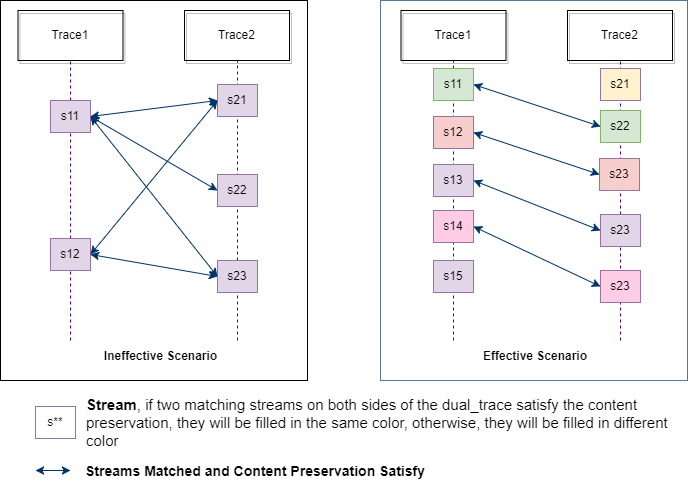
\includegraphics[scale=0.55]{Figures/secondlevelmatching}}
 \caption{Second Level Matching Scenarios}
\label{secondlevelmatching}
\end{figure}


The following subsections discuss the algorithms for these two level matching. In Section\ref{windows}, I elaborate the channel open process and the data transfer categories for the concerned communication methods. Based on the different channel opening process, two algorithms are developed for the communication identification, one is for Named Pipe and Message Queue, the other is for TCP and UDP. The inputs of the these two algorithms are the same, two $str$s from the original dual\_trace.

The data transfer characteristics divided the communication methods into reliable and unreliable transmissions. Named Pipe and TCP fall in the reliable category while Message Queue and UDP fall in the unreliable one. The second level matching algorithms are different for these two categories. The corresponding second level data verification algorithms are being used in the communication identification algorithms. The inputs of the transmitted data verification algorithms are streams matched in the first level matching while the output a boolean to indicate if the transmitted data of this two streams are matched and the verified data.

\subsection{Stream Matching Algorithm for Named Pipe and Message Queue}
For Named Pipe and Message Queue, only one channel open function is being called in each $s$. So in the below algorithm, when it try to get the channel open event from the $s.so$ list, only one event should be found and return. The channel identifier parameters can be found in the $ev.in$ of the channel open event. The identifier for Named Pipe is the file name of the pipe while for Message Queue is the format queue name of the queue. This algorithm finds out all the possible communications regardless some of them might be false negative errors. 

\begin{algorithm}[H]
\DontPrintSemicolon
\caption{{\bf Stream Matching Algorithm for Named Pipe and Message Queue} \label{channelAlg1}}
\KwIn{$str0, str1$}
\KwOut{$cs = \left\lbrace c_1, c_2...c_n\right\rbrace $}
$cs \leftarrow$ empty communication list;\;
\For{$s0 \in str0$}{
   $openev0 \leftarrow$ get the opening event from $s0.so$;\;
   $chId0 \leftarrow$ get the channel identifier from $openev0.in$;\;
   \For{$s1 \in str1$}{
      $openev1 \leftarrow$ get the opening event from $s1.so$;\;
      $chId1 \leftarrow$ get the channel identifier from $openev1.in$;\;
     \If{$chId0 == chId1$}{
         $DataVerified = dataVerify(s0, s1, outputdata)$;\;
         \If{$DataVerified == True$}{
            $c.stream0 = stream0$;\;
            $c.stream1 = stream1$;\;
            $c.dataMatch = outputdata$;\;
            $cs.add\left( c \right)$;\;
         }    
      }
   }
}
\KwRet $cs$;\;
\end{algorithm} 


\subsection{Stream Matching Algorithm for TCP and UDP}
For TCP and UDP multiple functions are collaborating to create the final communication channel. The local address and port of the server endpoint and the remote address and port of the client endpoint are used to identify the channel. This algorithm first try to retrieve the local address and port of the server endpoint and remote address and port from client endpoint. Then it try to match two endpoints by comparing the local and remote address and port. Transmitted data verification also applied in this algorithm.

\begin{algorithm}[H]
\DontPrintSemicolon
\caption{{\bf Stream Matching Algorithm for TCP and UDP} \label{channelAlg2}}
\KwIn{$str0, str1$}
\KwOut{$cs = \left\lbrace c_1, c_2...c_n\right\rbrace $}
$cs \leftarrow$ empty communication list;\;
\For{$s0 \in str0$}{
   $socketev0 \leftarrow$ get the $socket\left( \right)$ event from $str0.so$;\;
   $bindev0 \leftarrow$ get the $bind\left( \right)$ event from $str0.so$;\;
   $connectev0 \leftarrow$ get the $connect\left( \right)$ event from $str0.so$;\;
   \For{$s1 \in str1$}{
      $socketev1 \leftarrow$ get the $socket\left( \right)$ event from $s1.so$;\;
      $bindev1 \leftarrow$ get the $bind\left( \right)$ event from $s1.so$;\;
      $connectev1 \leftarrow$ get the $connect\left( \right)$ event from $s1.so$;\;
    \If{$socketev0 !=null$ AND $socketev != null$}{
       \If{$bindev0 != null$ AND $connectev1 == null$}{
           $localServerAddr \leftarrow$ get serverAddr from $bindev1.in$;\;
       }
       \ElseIf{$bindev1 == null$ AND $connectev0 != null$}{
           $remoteServerAddr \leftarrow$ get serverAddr from $connectev1.in$;\; 
       }
       \Else{
          Break the inner For loop;\;
       }
       \If{$localServerAddr == remoteServerAddr$}{
          $DataVerified = dataVerify(stream0, stream1, outputdata)$.
          \If{$DataVerified == True$}{
            $c.s0 = s0$;\;
            $c.s1 = s1$;\;
            $c.dataMatch = outputdata$; 
            $cs.add\left( c \right)$;\;
          }
       }
    }
   }
}
\KwRet $cs$;\;
\end{algorithm}

\subsection{Data Verification $dataVerify()$ for Named Pipe and TCP}
As described in Section\ref{reliable}, the data being received by one endpoint should always equal to or at least is sub string of the data being sent from the other endpoint in a communication for the reliable transmission methods, such as Named Pipe and TCP. So the data verification algorithm is in data union level. The send data union is retrieved by the concatenation of the input buffer content of the send events in the send stream of an endpoint. The receive data union is retrieved by the concatenation of the output buffer content of the receive events in the receive stream of the other endpoint. The input of this algorithm is the two $stream$s from two traces which are being matched in the first level.

\begin{algorithm}[H]
\DontPrintSemicolon
\caption{{\bf Transmitted Verification by Data Union} \label{dataAlg1}}
\KwIn{$s0, s1$}
\KwOut{send data union and receive data union of two streams}
\KwRet{Indicator of if transmitted data union are considered to be identical}\;
$send1 \leftarrow$ empty string;\;
$send2 \leftarrow$ empty string;\;
$recv1 \leftarrow$ empty string;\;
$recv2 \leftarrow$ empty string;\;
\For{$sendEvent \in s0.ss$}{
   $sendmessage \leftarrow$ get the input buffer content from the $sendEvent.in$;\;
   $send0.append\left( sendmessage \right)$;\;
}
\For{$sendEvent \in s1.ss$}{
   $sendmessage \leftarrow$ get the input buffer content from the $sendEvent.in$;\;
   $send1.append\left( sendmessage \right)$;\;
}
\For{$recvEvent \in s0.sr$}{
   $recvmessage \leftarrow$ get the output buffer content from the $recvEvent.out$;\;
   $recv0.append\left( sendmessage \right)$;\;
}
\For{$recvEvent \in s1.sr$}{
   $recvmessage \leftarrow$ get the output buffer content from the $recvEvent.out$;\;
   $recv1.append\left( sendmessage \right)$;\;
}
\If{$recv0$ is substring of $send1$ AND $recv1$ is substring of $send0$ }{
   \KwRet True;\;
}
\Else{
    \KwRet False;\;
}

\end{algorithm} 

\subsection{Data Verification $dataVerify()$ for MSMQ and UDP}
For the unreliable communication methods, the data packets being transmitted are not delivery and ordering guaranteed. So it is impossible to verify the transmitted data as a whole chunk. Fortunately, the packets arrived to the receivers are always as the original one from the sender. Therefore, we perform the transmitted data verification by single events instead of the whole stream. This algorithm basically goes through events of the $ss$ in one stream trying to find the matched receive event in the $sr$ in the other stream. And then calculate the fail packet arrival rate. The fail packet arrival rate should be comparable to the packet lost rate. So we set the packet lost rate as the threshold to determine if the transmitted data can considered to be identical in both directions. The packet lost rate can be various from network to network or even from time to time for the same network. The inputs of this algorithm are the copies of two streams from two traces which are being matched and the packet lost rate as the threshold. I use copies instead of original data is to modify the input list directly in the algorithm. The threshold should be an integer. For example if the lost rate is 5\%, the threshold should be set as 5. 

\begin{algorithm}[H]
\DontPrintSemicolon
\caption{{\bf Transmitted Verification by Data of Events } \label{dataAlg2}}
\KwIn{$s0, s1$}
\KwOut{matched event list of two endpoints}
\KwRet{Indicator of if transmitted data union are considered to be identical}\;
$sendPktNum0 \leftarrow s0.ss.length$;\;
$sendPktNum1 \leftarrow s1.ss.length$;\;
$recvPktNum0 \leftarrow 0$;\;
$recvPktNum1 \leftarrow 0$;\;
$eventMatchs \leftarrow List \langle EventMatch \rangle$;\;
\For{$sendEvent \in s0.ss$}{
   $sendmessage \leftarrow$ get the input buffer content from the $sendEvent.in$;\;
   \For{$recvEvent \in s1.sr$}{
      $recvmessage \leftarrow$ get the output buffer content from the $recvEvent.out$;\;
      \If{$sendmessage == recvmessage$}{
         $recvPktNum0++$;\;
         $stream1.sr.remove\left( recvEvent \right)$;\;
         $eventMatch = New eventMatch\left( \right)$;\;
         $eventMatchs.add\left( eventMatch \right)$;\;
      }
   }
}

\If{$ \left(sendPktNum0-recvPktNum0\right)*100/sendPktNum0 > threshold$}{
 \KwRet False;\;
}

\For{$sendEvent \in s1.ss$}{
   $sendmessage \leftarrow$ get the input buffer content from the $sendEvent.inputs$;\;
   \For{$recvEvent \in s0.sr$}{
      $recvmessage \leftarrow$ get the output buffer content from the $recvEvent.out$;\;
      \If{$sendmessage == recvmessage$}{
         $recvPktNum1++$;\;
         $s0.sr.remove\left( recvEvent \right)$;\;
      }
   }
}

\If{$ \left(sendPktNum1-recvPktNum1\right)*100/sendPktNum1 > threshold$}{
 \KwRet False;\;
}
 \KwRet True;\;
\end{algorithm}

\section{Relationship between Communication Model and Dual-Trace Model}
The identification of the communication from dual\_trace can be simply abstracted as finding the elements of each communication as defined in the communication model from the dual\_trace. 

A communication is defined as $c =<ch, e0, e1>$ while a dual\_trace is defined as $dtr = \lbrace tr0, tr1\rbrace$. In the dual\_trace model, a trace $tr$ can also be represented as stream trace $str = \lbrace s_1, s_2, ..., s_p\rbrace$. In the communication model, $ e =<handle, d_r, d_s>$. 

Each stream in $str$ contains four sub stream: $so, ss, sr, sc$.  The $handle$ of $e$ and $ch$ in $c$ can be acquired from the events in $so$. $d_r$ can be obtain from $sr$ while $d_s$ can be obtained from $ss$. And $pkg$ in the data stream in the communication model has a one to one relationship with $ev$ in the data send and receive stream in the dual\_trace model.

By understanding this relationship, I am optimistic that as long as I can retrieve all the elements defined in the trace in dual\_trace model, there will be a way to identify the communication. In next chapter algorithms for communication identification will be discussed in detail. 


\section{Communication Identification Algorithm}
The identification of the communications from a dual\_trace should be able to identify the concerned communications as well as all the components defined in it. The inputs of this algorithm are the $dual\_trace=\left\lbrace tr0, tr1 \right\rbrace $ and the concerned communication method's function set $fset = \left \lbrace f_1,f_2...f_m \right\rbrace $. The output of this algorithm is all the identified communications of the concerned communication method. This is a very high level algorithm, details of each step in this algorithm will be discussed in the later sections.\par
\begin{algorithm}[H]
\DontPrintSemicolon
\caption{{\bf Communication Identification Algorithm} \label{endpointIdentAlg}}
\KwIn{$dual\_trace$, $fset$}
\KwOut{$cs = \left\lbrace c_1, c_2...c_n\right\rbrace $}
$i = 0;$\;
\For{$tr \in dual\_trace$}{
   $etri = eventfilter\left( tr, fset\right)$;\;
   $stri = streamfilter\left( etr \right)$;\;
}
$cs = streammatch(str0, str1)$;\;
\KwRet $cs$;\;
\end{algorithm} 
